\documentclass[conference]{IEEEtran}

\usepackage{cite}
\usepackage{amsmath,amssymb,amsfonts}
\usepackage{algpseudocode}
\usepackage{algorithm}
\usepackage{graphicx}
\usepackage{textcomp}
\usepackage{xcolor}
\def\BibTeX{{\rm B\kern-.05em{\sc i\kern-.025em b}\kern-.08em
    T\kern-.1667em\lower.7ex\hbox{E}\kern-.125emX}}
\begin{document}

\title{Forest Cover Classification\\

}

\author{\IEEEauthorblockN{DT Nicolay 26296918}
\IEEEauthorblockA{\textit{Department of Computer Science} \\
\textit{Stellenbosch University}\\
Stellenbosch, South Africa \\
26296918@sun.ac.za}
}

\maketitle

\begin{abstract}
This document is a model and instructions for \LaTeX.
This and the IEEEtran.cls file define the components of your paper [title, text, heads, etc.]. *CRITICAL: Do Not Use Symbols, Special Characters, Footnotes, 
or Math in Paper Title or Abstract.
\end{abstract}

\begin{IEEEkeywords}
component, formatting, style, styling, insert.
\end{IEEEkeywords}

\section{Introduction}
introooo TODO remove
``Fig.~\ref{fig}'', even at the beginning of a sentence.

\begin{table}[htbp]
\caption{Table Type Styles}
\begin{center}
\begin{tabular}{|c|c|c|c|}
\hline
\textbf{Table}&\multicolumn{3}{|c|}{\textbf{Table Column Head}} \\
\cline{2-4} 
\textbf{Head} & \textbf{\textit{Table column subhead}}& \textbf{\textit{Subhead}}& \textbf{\textit{Subhead}} \\
\hline
copy& More table copy$^{\mathrm{a}}$& &  \\
\hline
\multicolumn{4}{l}{$^{\mathrm{a}}$Sample of a Table footnote.}
\end{tabular}
\label{tab1}
\end{center}
\end{table}

\begin{figure}[htbp]
\centerline{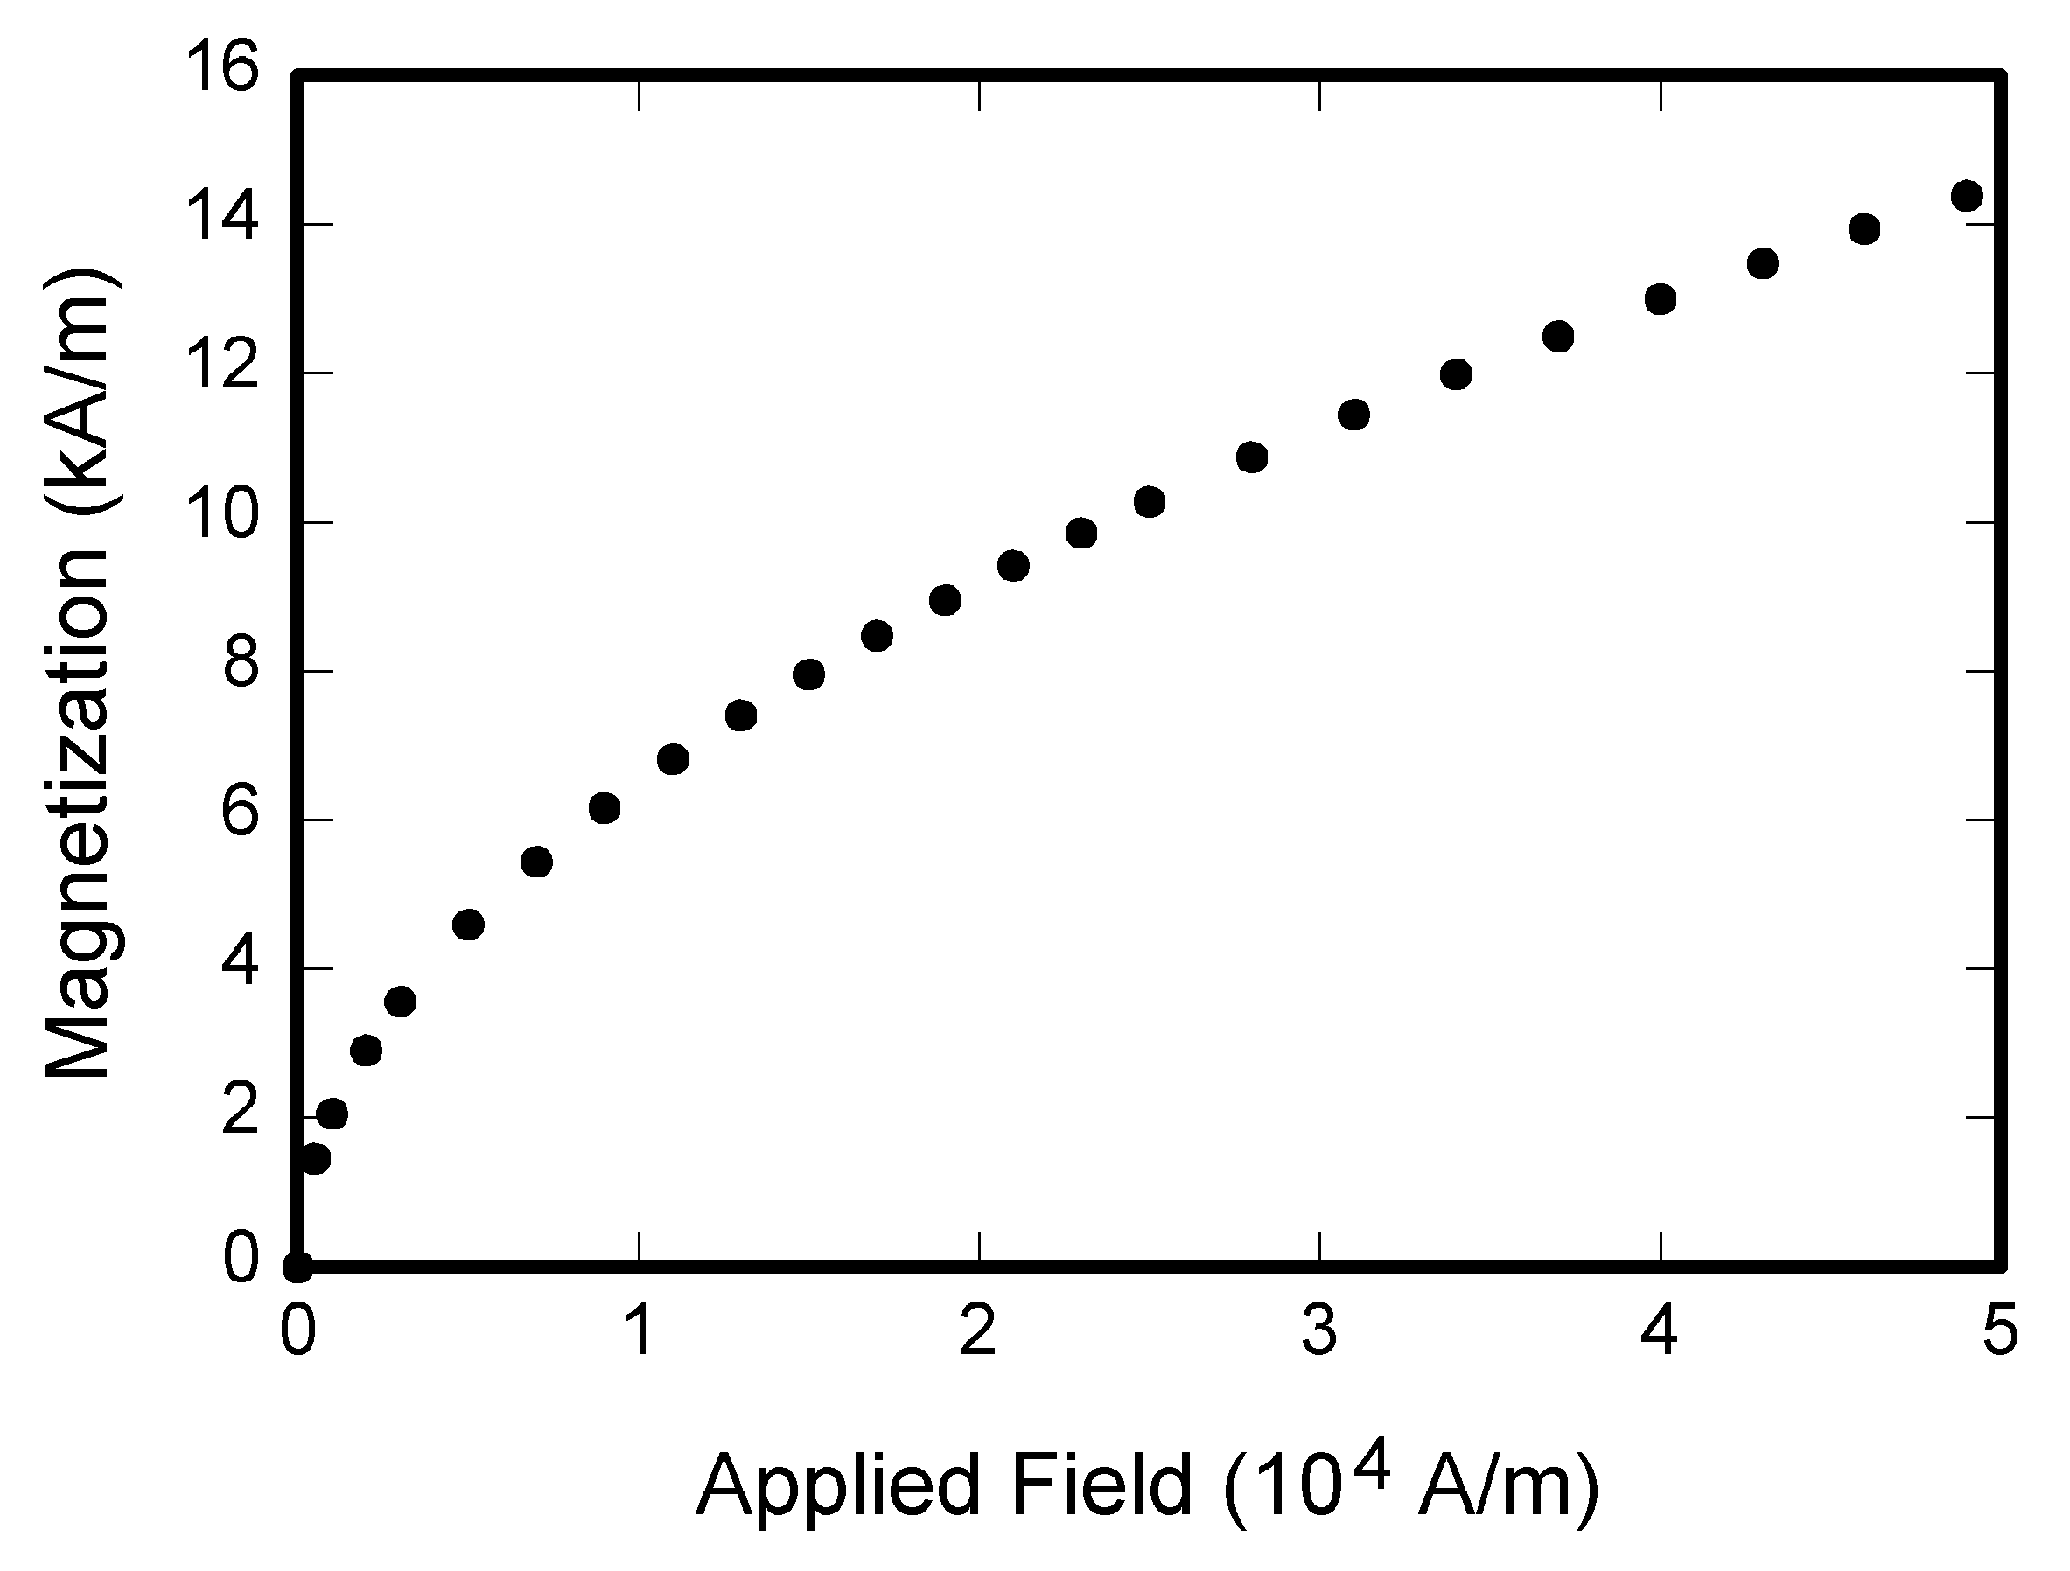
\includegraphics{fig1.png}}
\caption{Example of a figure caption.}
\label{fig}
\end{figure}

Figure Labels: Use 8 point Times New Roman for Figure labels. Use words 
rather than symbols or abbreviations when writing Figure axis labels to 
avoid confusing the reader. As an example, write the quantity 
``Magnetization'', or ``Magnetization, M'', not just ``M''. If including 
units in the label, present them within parentheses. Do not label axes only 
with units. In the example, write ``Magnetization (A/m)'' or ``Magnetization 
\{A[m(1)]\}'', not just ``A/m''. Do not label axes with a ratio of 
quantities and units. For example, write ``Temperature (K)'', not 
``Temperature/K''.

\section{Introduction}
\section{Background}

\subsection{k-nearest Neighbours (kNN)}
The nearest neighbour algorithm is an example of instance-based learning where the prediction for an instance is made by comparing the instance to similar training instances. This is a lazy learning approach since we delay processing training data until prediction is needed \cite{kelleher2020fundamentals}. Since kNN is also similarity-based, it is non-parametric, which means that it does not learn a mapping from the input space to the output space.

The k-nearest neighbour algorithm is presented in Algorithm~\ref{alg:knn} which explains that we calculate the distance from each data point in our training dataset to the distance. From there, we choose the closed \textit{k} observations and perform inference. In a classification context we may perform majority voting to determine the class, in a regression context we use the mean or median of the \textit{k} nearest observations.

In order to use the algorithm we need to define a value of \textit{k} which decides the number of nearest neighbour instances to consider when predicting. Choosing a value a low value for \textit{k} results in a high variance, but low bias leading to an unstable model which tends to overfit. Choosing a large value for \textit{k} results in a smaller variance, but high bias, leading to a more stable model which tending to underfit. Measures such as \textit{k}-fold cross validation assist in the selection of a value of \textit{k}.

\begin{algorithm}[htbp]
\caption{k-Nearest Neighbors Algorithm}
\label{alg:knn}
\begin{algorithmic}
\Function{kNN}{$D, x, k$}
\ForAll{$x' \in D$}
\State $d = \text{distance}(x, x')$
\EndFor
\State sort($d$)
\State $S = $ set of $k$ patterns in $D$ closest to $x$
\State \Return class as majority class in $S$
\EndFunction
\end{algorithmic}
\end{algorithm}
\noindent
\textbf{Notation:} $D$ denotes the training dataset, $x$ is the query instance, $k$ is the number of nearest neighbours, and $\text{distance}(\cdot)$ is a distance metric (e.g., Euclidean distance).

Another important part in the kNN algorithm is the distance metric. This determines how similarity between observations is measured. Euclidean distance is the most common metric. It calculates the line distance between two points in space, this is useful for continuous numerical features. Manhattan distance computes the sum of absolute differences across each dimension. It is often used when features are not strongly correlated. A generalization of these two is the Minkowski distance, which introduces a parameter \(p\) that allows interpolation between different norms: when \(p = 1\), it reduces to Manhattan distance, and when \(p = 2\), it becomes Euclidean distance. The choice of metric can significantly impact the performance of kNN, especially in high-dimensional spaces or when feature scales differ.

\subsection{Classification Trees}
Classification trees represent a fundamental approach in supervised machine learning for predictive modelling, where the learned model forms a hierarchical tree structure with non-terminal nodes representing decisions on descriptive features and terminal leaf nodes representing target feature predictions \cite{quinlan1993c45}. A classification tree is a type of decision tree where leaf nodes represent different discrete classes.

Classification trees employ recursive partitioning where a training dataset is systematically divided into increasingly homogeneous subsets based on feature values. It uses a greedy strategy to select the feature to partition upon at each split that maximises information gain \cite{kelleher2020fundamentals}. The information gain criterion, derived from Shannon's entropy measure, quantifies the reduction in uncertainty achieved by partitioning the data according to a specific feature test.
Formally, given a dataset $D$ with $M$ different classes, the entropy is calculated as:

\[
H(D) = -\sum_{m=1}^{M} p(y_m) \log_{M} p(y_m)
\]

where $p(y_m)$ represents the probability of class $y_m$ occurring in $D$. When the dataset is partitioned on feature $\alpha$ into $O$ outcomes, the information gain is computed as:

\[
\text{gain}(\alpha) = H(D) - H_\alpha(D)
\]

where 

\[
H_\alpha(D) = \sum_{o=1}^{O} p_o \, H(D_o)
\]

represents the weighted entropy after the split.

Since we recursively partition until either a stopping condition is satisfied or all subsets are homogeneous, classification trees inherently lead to overfitting, as the algorithm attempts to perfectly classify all training instances, often creating overly complex trees that capture noise rather than underlying patterns \cite{quinlan1993c45}. To remedy this, post-pruning techniques are used to remove branches that do not improve generalisation performance.

Classification trees can naturally handle both categorical and numerical features. Classification tree induction algorithms can cope with missing values. Unfortunately, classification trees exhibit an axis-aligned bias which restricts decision boundaries to be parallel to feature axes.

\subsection{Expectations With Respect to Data Quality Issues}
Since kNN relies heavily on distance metrics, it will be severely impacted by missing values since it cannot compute meaningful distances between points. This can however be handled by ignoring the missing values in the distance calculation and scaling up the weight of the non-missing descriptive features. The kNN algorithm can actually be used as an imputer itself as well. If nothing is done the algorithm will either fail or give biased distances. Classification trees on the other hand handle missing values more gracefully. Classification trees can adjust the gain ratio calculation 
\[
\text{gainRatio}(x) = (1 - F) \times \big( H(D) - H_x(D) \big)
\]

\text{where } F \text{ is the fraction of missing patterns.}



With regards to the Facet feature being correlated with the Aspect feature, kNN will be moderately impacted since the distance calculation used will overweight certain areas of similarity. There is no built in mechanism to handle feature correlation as a data issue. Classification trees will be minimally impacted since trees naturally handle correlated features through the feature selection process involving the gain ratio/information gain. This means that the classification tree induction will likely select one feature and ignore the correlated redundant one.

Concerning the Inclination feature only containing noisy values, the impact on the kNN algorithm will depend on the value of \textit{k} since higher values are more sensitive to noise and lower values are more robust to noise. However, since there are many predictive features the value won't dominate the distance calculation. Classification trees are robust to noise and will handle it through pruning. The noisy patterns will end up in small leaf nodes as the model overfits and post-pruning removes these leaves. The noise becomes a minority and does not affect majority class prediction.

Since kNN employs distance measures which are often sensitive to outliers since the distance can be seriously skewed even if only one feature is outlying. For small values of \textit{k} outliers are unlikely to be nearest neighbours and will therefore have limited influence. For large values of \textit{k} the outliers will also have limited influence due to majority voting. Cumulatively, outliers will have a moderate impact on the kNN algorithm. Classification trees are robust to outliers since they handle them in a similar way to noise. Outliers are first isolated in small leaf nodes during induction. Pruning removes leaves which contain outliers which results in outliers becoming a minority in combined larger subsets. This makes decision trees robust to outliers.

The kNN algorithm will be severly impacted from features with numeric ranges that differ significantly from one another since features with large ranges dominate distance calculations. For example, if one feature takes on the value of 0 or 1 and another takes on the value of 0 or 100 000, the second will overwhelm the distance calculation. Without normalisation, the kNN algorithm will be unreliable. Classification trees have a natural robustness to different feature scales and therefore will be minimally impacted. This stems from trees using individual feature values for splitting thresholds.

The mixed data types will affect the kNN algorithm since it requires special handling for mixed types such as using the Gower's similarity with different similarity measures for different types. However, in this dataset since there are two categorical variables with the first encoded over four columns and the second over 40 and 13 numeric features there can be a distance bias toward the numeric features. Euclidean distance assumes features are continuous, but the categorical features are encoded as zero or one. Classification trees naturally handle mixed data types since they directly compare categorical features against each other for splitting, and the splitting is simply decided off information gain.

The impact of the Water Level feature having a cardinality of one will be none at all for kNN. It will only contribute the the distance calculation unnecessarily and be a computational waste. Since all observations have the same value, all the distance measures will be equally skewed, resulting in no impact at all. The classification tree will never select this feature during tree indication since there is zero information gain because all values are identical. Therefore, classification trees naturally handle this issue and it will have no impact.

The Observation ID unique feature will have a sever impact on kNN since each instance appears maximally different from all others on this feature. The problem is that this dominates distance calculations making all instances seem dissimilar. It breaks the fundamental assumption of similarity-based learning. Classification trees will overfit severely since each unique value would create a separate branch. The information gain maximisation favours features with many outcomes so the result will be an extremely busy tree with poor generalisation.

The skewed class distribution impact on kNN depends on the value of \textit{k}, since a smaller \textit{k} is more robust to class imbalance whilst a large \textit{k} results in the majority class dominating the predictions. Methods such as the Synthetic Minority Over-sampling Technique (SMOTE) must be considered. The impact of classification trees is moderate since they are sensitive to skewed distributions. The minority class instances result in small leaves which are likely to be pruned, then the combined instances will be classification as a majority class. This results in poor minority class recognition.

\section{Methodology}
\subsection{Tools and Libraries}
This implementation was created using Python. NumPy was used for numerical computations. Pandas was used for data manipulation and analysis. Matplotlib was used for data visualisation and plotting. Seaborn was used for statistical data visualisation. Scikit-learn was used extensively for pre-processing, model selection, validation, both machine learning algorithms, and the evaluation metrics. The imbalanced-learn library was used for the SMOTE and Tomek techniques. For statistical testing, SciPy was used.
\section{Empirical Procedure}

\subsection{Data Pre-processing}
In this section we discuss the data pre-processing steps applied to the dataset prior to implementing the k-nearest neighbour and classification tree algorithms.
\subsubsection{k-Nearest Neighbour Data Pre-processing}
First, the unique identifier feature \texttt{Observation\_ID} was removed because unique values make all instances appear maximally different. This breaks the similarity-based learning assumptions and leads to the feature dominating distance calculations. The feature has no signal that can provide the model with any benefit.

Second, we removed the constant feature \texttt{Water\_Level} since it provides zero discriminative information but adds computational overhead to all the distance calculations. We can be certain that the model performance will not change based on the fact that the feature has a cardinality of one.

Third, we normalised the numeric features by applying linear scaling to ensure the numeric features are in the same range being between zero and one. Features with large ranges will simply dominate distance calculations over smaller range features. This would make the model unreliable and heavily weight features with higher values. Specifically, \texttt{Elevation}, \texttt{Aspect}, \texttt{Slope}, \texttt{Horizontal\_Distance\_To\_Hydrology}, \texttt{Vertical\_Distance\_To\_Hydrology}, \texttt{Horizontal\_Distance\_To\_Roadways}, \texttt{Hillshade\_9am}, \texttt{Hillshade\_Noon}, \texttt{Hillshade\_3pm}
 are all normalised.
 
 Fourth, we handled the missing values by using kNN imputation with a \textit{k} of five. There are only 298 observations that are missing the \texttt{Slope} feature. For each of these we computed the Euclidean distance between the observation and all others based on available features, then identified the \textit{k} closest rows (neighbours) that have the missing feature value. The mean of these values were calculated and imputed to the missing observation.
 
 Fifth, we addressed the feature correlation issue by removing the \texttt{Facet} feature since it is just providing redundant information. Correlated features can overweight certain aspects in distance calculations resulting in worse model performance. Essentially, the \texttt{Aspect} feature would have double the influence on the model as the other features if \texttt{Facet} was not removed.
 
 Sixth, the mixed data types issue was handled by converting the one categorical variable \texttt{Soil\_Type1} to numeric. This was achieved by simply replacing all the instances with a \textit{positive} value with the number one, and the \textit{negative} instances with zero. This approach was chosen since it aligned the feature with the other soil type features which all take on the values of either one or zero.
 
 Seventh, the features containing outliers were left untouched. The kNN algorithm has moderate sensitivity to feature-based outliers, but a small \textit{k} value provides natural protection.
 
 Eighth, SMOTE was used to improve the class imbalance. Since the five minority classes had significantly fewer observations than the majority two classes, we employed SMOTE to increase the number of minority class observations to 20\% of the majority class. This partial balancing approach was used since the dataset only increased in size by 34\%, as opposed to the dataset exploding in size if they were all were made equal. For example, if we over-sample class 4 to 283,301 we'd create 280 000 synthetic samples for one class. This is massive and risky for overfitting. On top of this Tomek links for majority class under-sampling was also used to reduce the number of observations in the majority classes. Using this under-sampling technique alone would not be sufficient since only a small fraction of the majority samples are removed. The Tomek link technique resulted in the majority classes reducing by roughly 60 000 observations in each majority class. That is, Class 1 now has 158,427 samples, and Class 2 now has 225,918 samples after reduction.  It is important to note that SMOTE was only applied to the \textit{training} datasets and never to the \textit{test} datasets.
 
 Ninth, the noisy feature \texttt{Inclination} was removed since it was confirmed to contain only noise. Noisy features affect distance calculations, although larger \textit{k} values provide some robustness it is safer to remove it since we know it contains no signal.

\subsubsection{Classification Trees Data Pre-processing}

First, the unique identifier feature \texttt{Observation\_ID} was removed because it creates severe overfitting. Classification tree induction will result in one branch per unique value in this feature, this triggers the many-values bias in information gain maximisation. Again, since the feature provides no predictive power we can safely remove it without losing anything important.

Second, the constant \texttt{Water\_Level} feature was removed since it will always result in zero information gain if the classification tree were to split on it. The algorithm will naturally ignore it, but it does waste computational resources.

Third, the target class imbalance was addressed using SMOTE to over-sample the minority classes. Again, the minority classes were over-sampled to 20\% of the size of the largest majority class. This is done because trees are sensitive to skewed distributions since minority classes get pruned away leading to poor recognition. To use SMOTE, the missing values needed to be temporarily imputed using kNN imputation and the categorical variables encoded. This was performed to enable SMOTE to work as intended. The classification tree was still trained on the dataset containing missing values and categorical features. It is important to note that SMOTE was only applied to the \textit{training} datasets and never to the \textit{test} datasets.

Fourth, the missing values were left as is since the classification trees have excellent built-in missing value handling. Pre-processing is therefore unnecessary in this case. The tree induction algorithm distributes the instance fractionally across all branches where a feature is missing, this is done proportional to the observed frequencies of those branches among the non-missing data.

Fifth, the correlated \texttt{Facet} and \texttt{Aspect} features are left as is. Trees naturally handle correlation through information gain and redundant features are automatically ignored. The algorithm will select the most informative feature.

Sixth, the mixed data types are left as is. Classification trees natively handle both categorical and numeric features without the need for conversion.

Seventh, the numerical feature scale differences need not be attended to. Trees are scale-invariant since they use a threshold-based split that works regardless of the feature ranges. The features are only compared on an information gain basis and not by their values. This is unlike the kNN algorithm which compares the values of the features during the distance measurements.

Eighth, the outliers are left in the dataset. Classification trees are naturally robust to outliers through the pruning process. The C4.5 algorithm \cite{quinlan1993c45} uses error-based pruning. If a branch only exists because of a few outliers, that branch has few training examples. Therefore, its estimated error rate is high.

Ninth, the noisy feature \texttt{Inclination} is kept since the pruning process handles noise. Trees handle noise well by isolating noisy patterns in small leaves that get pruned.


\subsection{Control Parameter Tuning}
In this section we discuss the custom cross-validation approach used to tune the parameters for each of the algorithms. The key principle is that the SMOTE/Tomek techniques are only applied to training folds, never to validation folds, ensuring realistic performance estimates.
\subsubsection{k-Nearest Neighbour Control Parameter Tuning}
The three primary parameters were optimised over during a 5-fold stratified cross-validation on a 20\% subset for computational efficiency. First, is the value of \textit{k} which controls the number of nearest neighbours to consider. Values of [3, 5, 7, 9, 11, 15] were considered. Second, both the options for the weights parameter were considered. Specifically, uniform where all neighbours are weighted equally and distance weighting where closer neighbours have more influence. Third, three distance metrics were considered: Euclidean distance, manhattan distance, and minkowski distance (which is a generalisation of both with a \textit{p} parameter). Since there are three parameters with six, two, and three options respectively, there are $6 \times 2 \times 3 = 36$ parameter combinations to test in the cross-validation. 
	
\subsubsection{Classification Trees Control Parameter Tuning}
The five primary parameters were optimised over during a 5-fold stratified cross-validation on a 20\% subset for computational efficiency.  First, four maximum depth parameter values were considered: [10, 15, 20, 25]. This parameter controls tree depth to balance complexity against generalisation. Second, the minimum number of samples required to split an internal node. The values of [2, 5, 10, 20] were considered. Higher values prevent overfitting by requiring more evidence for splits. Third, the minimum number of samples required at leaf nodes was tuned, with values of [1, 2, 5, 10]. This prevents the formation of overly specific rules that do not generalise well. Fourth, the splitting criterion was evaluated using both \textit{gini} (Gini impurity) and \textit{entropy} (information gain). Gini is computationally faster, while entropy provides a more theoretically principled approach. Finally, the \textit{max\_features} parameter was tuned over ['sqrt', 'log2', None], which controls the number of features considered for the best split. Using \textit{sqrt} or \textit{log2} introduces randomness to improve generalisation, while None considers all features. Since there are five parameters with four, four, four, two, and three options respectively, there are $4 \times 4 \times 4 \times 2 \times 3 = 384$ parameter combinations tested. 


\subsection{Performance Metrics}
Four primary metrics were considered to evaluate the performance of the models. Accuracy was used to evaluate the overall correctness of predictions across all classes.  Macro and weighted precision was used to evaluate the algorithm's ability to avoid false positives. Macro and weighted recall was used to test the algorithm's ability to find all positive cases. F1-Score was also employed as a measure of the algorithm's overall performance. 

Ten-fold cross-validation mean accuracy was employed to provide robust performance estimation. The standard deviation of the cross-validation score was used to measure the algorithm stability across the various folds. The range of the cross-validation scores was also evaluated to show the best and worst fold performance. 

Statistical testing using t-tests and 95\% confidence intervals quantified significance and uncertainty. Computational metrics such as training time, prediction time, and model complexity (e.g., parameter count, tree depth, memory usage) were also recorded. Weighted averages were applied to handle class imbalance, and multiple metrics were used to avoid over-reliance on a single measure.

\subsection{Analysis Process}
Proper train/test methodology was used to prevent data leakage. Specifically, the SMOTE and Tomek techniques were only applied to the training dataset and not the test or validation datasets. This ensures that the test sets have not synthetic data and that they are raw.

A custom cross-validation implementation was employed to ensure proper resampling and that the SMOTE and Tomek techniques were only applied within each \textit{training} fold. The validation was unbiased since it was performed on the original unbalanced data.

TODO add learning curve analysis

Statistical significance testing was used to perform a rigorous comparison through the t-test to determine if performance differences in the cross-validation are meaningful. Confidence intervals were used to provide uncertainty bounds around estimates.
TODO finish

\section{Research Results}
\section{Conclusion}
\section*{References}

\bibliographystyle{IEEEtran}
\bibliography{references}

\end{document}
